\documentclass{article}
\usepackage{enumitem}
\usepackage{graphicx}
\usepackage[letterpaper, margin=1in]{geometry}
\usepackage{times}
\usepackage{newtxtext}
\usepackage{multicol}  % Add this line for the multicol package
\usepackage{natbib}  
\usepackage{hyperref} 

\begin{document}

\begin{titlepage}
    \centering
    
\includegraphics[width=0.6\textwidth]{images/logo.png}
    
    \vspace{2cm}

    {\fontsize{24pt}{28.8pt}\selectfont \fontfamily{ptm}\selectfont \textbf{Optimizing Home Energy Management: The Transformative Role of Progressive Web Apps (PWA) in Residential Electrical Measurements}}
    \vspace{1cm}
    
    {\Large Made by:}

    \vspace{1cm}

    {\fontsize{10pt}{28.8pt}\selectfont Gomez Leyva Jesus Armando}

    \vspace{0.5cm}
    {\fontsize{10pt}{28.8pt}\selectfont Luna Perez Cristian}

    \vspace{0.5cm}
    {\fontsize{10pt}{28.8pt}\selectfont Moreno Maya Marco}

    \vspace{0.5cm}
    {\fontsize{10pt}{28.8pt}\selectfont Labrada Galvez Antonio}
    
    \vspace{2cm}
    
    {\large January 17th, 2024}
    
\end{titlepage}

\begin{multicols}{2}  % Start two-column layout

\section*{Executive Summary}
This document explores the integration of Progressive Web Apps (PWA) into residential electrical measurement applications, offering an efficient and accessible solution to empower users in monitoring and managing their energy consumption.

\section*{Introduction}
With the rise of connected devices in homes, residential electrical measurement has become more crucial than ever. However, traditional applications often lack accessibility and advanced features. The adoption of PWA is presented as an innovative solution to enhance the user experience in this context.

\section*{Problem Description}
Conventional home electrical measurement applications are often limited in terms of accessibility, automatic updates, and performance. These challenges impact users' ability to understand and efficiently manage their energy consumption.

\section*{PWA in Residential Electrical Measurement}
A detailed exploration of how Progressive Web Apps can address current limitations in residential electrical measurement applications, providing quick and easy access from any device, even in environments with variable connectivity.

\begin{itemize}
    \item \textbf{Offline Accessibility:} Progressive Web Apps enable users to access residential electrical measurement data even without a continuous internet connection, ensuring usability in various scenarios.
    \item \textbf{Automatic Updates:} PWAs can seamlessly update to reflect changes in rates, regulations, or additional features, ensuring users always have the latest information at their fingertips.
    \item \textbf{Cross-Device Compatibility:} With PWA, users can monitor their energy consumption from a range of devices, including smartphones, tablets, and desktop computers, enhancing accessibility and convenience.
\end{itemize}

\section*{Practical Use Cases}
Examples illustrating how PWAs can be used in everyday situations, enhancing the experience of residential electrical measurements:

\begin{enumerate}
    \item \textbf{Remote Monitoring:} Utilize the PWA to remotely monitor real-time energy consumption from a mobile device, providing users with instant access to their home's electrical data.
    
    \item \textbf{Alerts for Consumption Peaks:} Implement an alert system within the PWA to notify users when their energy consumption exceeds predefined thresholds. This feature empowers users to take immediate actions in response to unexpected spikes in usage.
    
    \item \textbf{Detailed Energy Usage Analysis:} Enable users to conduct in-depth analyses of their energy usage patterns through the PWA. Utilize interactive graphs and charts to present historical data, helping users make informed decisions about energy-saving strategies.
\end{enumerate}

\section*{Advantages and Benefits}
\begin{itemize}
    \item \textbf{Accessibility from Mobile Devices:} Users can access the residential electrical measurement application from various mobile devices, providing convenience and flexibility.
    
    \begin{figure*}
        \centering
        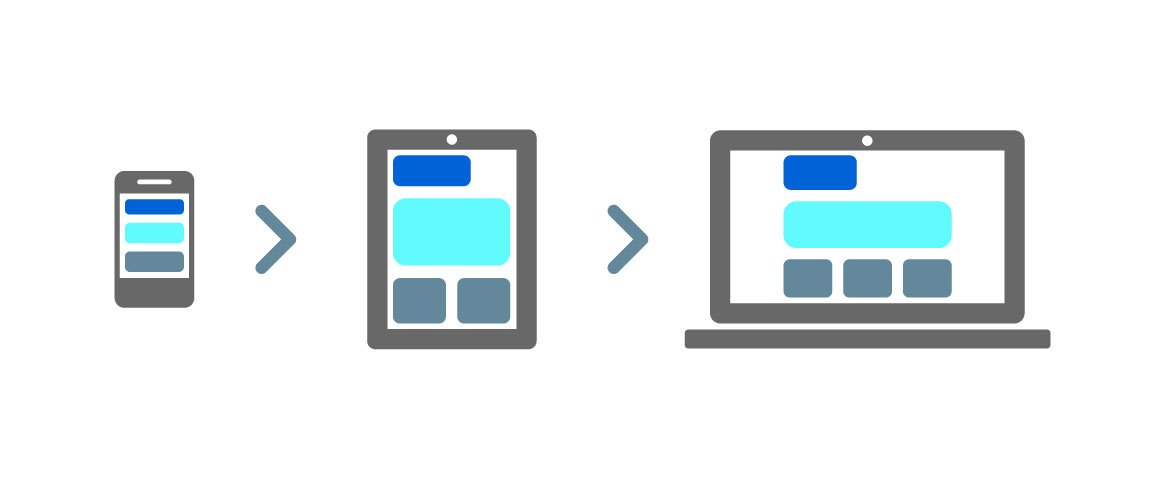
\includegraphics[width=0.8\textwidth]{images/mobile-first.jpg}  % Adjust the width as needed
        \caption{PWA allows you to use your application across all devices.}
    \end{figure*}

    \item \textbf{Automatic Updates:} Progressive Web Apps (PWA) allow for automatic updates, ensuring that the application reflects changes in rates and features without requiring manual intervention from users.
    
    \item \textbf{Offline Access to Consumption Data:} PWAs enable users to access their energy consumption data even in offline mode, ensuring uninterrupted insights into their usage patterns.
    
    \item \textbf{Improved Performance:} PWA's ability to cache resources intelligently results in improved performance, particularly in environments with variable connectivity, enhancing the overall user experience.
    
    \item \textbf{Enhanced User Engagement:} The accessibility and user-friendly nature of PWAs contribute to increased user engagement, fostering a deeper understanding of energy consumption and encouraging users to make informed decisions.
\end{itemize}



% Continue the rest of your document...


\section*{Security and Privacy}
Addressing concerns about data security and privacy is paramount in the implementation of Progressive Web Apps (PWAs) for residential electrical measurement. The following considerations demonstrate how PWAs can implement robust security measures and respect user privacy:

\begin{itemize}
    \item \textbf{Data Encryption:} Ensure that all communication between the PWA and the backend servers is encrypted using secure protocols such as HTTPS. This prevents unauthorized access to sensitive user data during transmission.

    \item \textbf{Authentication Mechanisms:} Implement strong user authentication mechanisms to verify the identity of users accessing the PWA. This can include multi-factor authentication for an additional layer of security.

    \item \textbf{Secure Storage:} Utilize secure storage mechanisms for storing sensitive data on the user's device. This helps protect user information even in the event of device loss or theft.

    \item \textbf{Privacy by Design:} Design the PWA with privacy in mind, following the principles of privacy by design. Minimize data collection to only what is necessary for the application's functionality, and obtain user consent for data processing.

    \item \textbf{User Consent and Transparency:} Clearly communicate to users about the types of data collected, how it will be used, and obtain explicit consent. Users should have control over their data and be informed about any changes in privacy policies.

    \item \textbf{Regular Security Audits:} Conduct regular security audits to identify and address potential vulnerabilities. Keep the PWA and associated systems up-to-date with the latest security patches.

    \item \textbf{Legal Compliance:} Ensure compliance with relevant data protection regulations and laws. This may include GDPR, CCPA, or other regional privacy regulations depending on the user base.
    
    \vspace{0,5cm}
    \citep{Security}
\end{itemize}

\section*{Conclusions}
In conclusion, the integration of Progressive Web Apps (PWAs) into residential electrical measurement applications represents a transformative step towards enhancing user experience and promoting efficient energy management. By addressing the limitations of traditional applications, PWAs offer quick and accessible access to consumption data, automatic updates, and offline functionality.

\vspace{0,5cm}

The advantages and benefits of implementing PWAs in this context, such as improved accessibility from mobile devices and real-time updates reflecting changes in energy rates, contribute to empowering users in their efforts to monitor and manage energy consumption effectively. Practical use cases demonstrate the versatility of PWAs, enabling remote monitoring, timely alerts for consumption peaks, and detailed analysis of energy usage within the home.

\vspace{0,5cm}

Security and privacy considerations have been thoroughly addressed, assuring users that the implementation of PWAs in residential electrical measurement applications prioritizes robust security measures and respects user privacy.

\vspace{0,5cm}

In summary, the adoption of PWAs offers a holistic solution to the challenges faced by conventional applications, enabling users to make informed decisions, enhancing energy efficiency, and ultimately transforming the way residential energy consumption is monitored and managed.
\section*{Recommendations}
Suggestions on how utility providers and developers can adopt PWA in their residential electrical measurement applications, offering an enhanced experience for end-users.

\bibliographystyle{plainnat} % Choose a bibliography style
    \bibliography{references.bib} 
\end{multicols}  % End two-column layout
\end{document}
